\documentclass[conference]{IEEEtran}
\IEEEoverridecommandlockouts
\usepackage[T1]{fontenc}
\usepackage{cite}
\usepackage{amsmath,amssymb}
\usepackage{booktabs}
\usepackage{graphicx}
\usepackage{xcolor}
\usepackage{url}
\usepackage[hidelinks]{hyperref}
\usepackage{multirow}
\usepackage{siunitx}

\newcommand{\todo}[1]{\textcolor{red}{[TODO: #1]}}
\newcommand{\pv}[1]{$p{=}#1$}

\title{Skill-Level Experts with Grounded Targets:\\
Modularity, Generality and Reliability in\\Language-Conditioned Manipulation}
\author{\IEEEauthorblockN{Prateek Pawar}
\IEEEauthorblockA{Independent researcher\\
prateekspawar@gmail.com}}

\begin{document}
\maketitle

\begin{abstract}
Vision-language-action (VLA) models are increasingly specialised by attaching small task-specific experts to a
shared, frozen backbone. We ask at which granularity such experts should be defined. We compare three ways of
organising the same model capacity, data and compute for language-conditioned pick-and-place on a 5-DoF arm in
simulation: one monolithic model, \emph{task-level} experts (one per instruction, as in recent LoRA-expert
systems), and \emph{skill-level} experts (one per primitive---find, pick, place, stack---composed into tasks),
all conditioned on a target pose provided by an open-vocabulary perception and tracking stack. In seeded, paired
evaluations of 50--150 episodes per condition we find that (i) splitting by skill does not improve per-skill
accuracy over a monolithic model trained on the same data; (ii) skill-level experts generalise far better than
task-level experts, on seen (90--98\% vs.\ 56--72\% success) and unseen instructions (94\% vs.\ 48--58\%), because
every skill learns from all episodes; (iii) a new skill can be added in isolation without any access to old data
or risk to deployed skills, while naive fine-tuning of a monolithic model erases its previous skills (0\%), and
fine-tuning with replay retains them but requires the old data and full re-validation. We further report a
failure-driven reliability study in which executor-level mechanisms---a proprioceptive grasp check with retry and
a release gate---raise end-to-end success from 45\% to 91\% (and from 22\% to 87\% under object pushes), more than
any model change. On unseen multi-step tasks, skills compose almost independently for both organisations, and
composite success is bounded by the weakest skill, here stacking onto raised targets.
\end{abstract}

\begin{IEEEkeywords}
vision-language-action models, modular policies, skill composition, imitation learning, robot manipulation
\end{IEEEkeywords}

%======================================================================
\section{Introduction}
%======================================================================
\begin{figure*}[t]
\centering
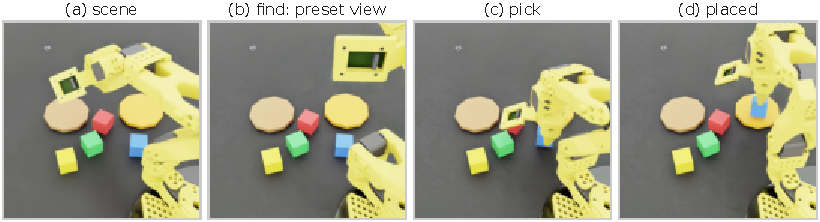
\includegraphics[width=\textwidth]{figures/fig_scene.pdf}
\caption{A successful evaluation episode seen from the left head camera: ``put the blue cube on the orange plate''.
(a) Initial scene with randomly coloured plates; (b) \texttt{find} looks from a preset viewpoint; (c) \texttt{pick}
grasps the tracked cube; (d) \texttt{place} releases it on the plate.}
\label{fig:scene}
\end{figure*}
Generalist VLA policies such as OpenVLA~\cite{kim2024openvla}, $\pi_0$~\cite{black2024pi0} and
SmolVLA~\cite{shukor2025smolvla} map images and an instruction to robot actions. Adapting them to new tasks
without degrading old ones is an open problem: fine-tuning one model on new data causes interference and
forgetting~\cite{mccloskey1989catastrophic}. A recent and effective answer is to freeze the backbone and attach a
lightweight expert per task, selected at run time from the instruction~\cite{luo2026coral}.

This raises a design question that, to our knowledge, has not been studied in a controlled way: \emph{what should
an expert be responsible for?} Experts can be defined per task (``put the blue cube on the blue plate'') or per
skill (``pick'', ``place''), with a planner composing skills into tasks~\cite{ahn2022saycan,liang2023cap}. The
two choices partition the same data very differently. A task expert sees only the demonstrations of its
instruction; a skill expert sees the corresponding segment of every demonstration, regardless of which objects are
involved---provided it is told \emph{which} object to act on. We provide that information explicitly as a target
pose from an open-vocabulary detection, stereo and tracking stack, building on evidence that grounded 3-D targets
strongly improve VLA generalisation~\cite{stone2023moo,tsai2026headinjection}.

Figure~\ref{fig:organisation} contrasts the three organisations we compare.

\paragraph{Contributions.}
\begin{itemize}
\item A modular architecture of skill-level experts on a shared frozen VLA backbone, each conditioned on a tracked
  9-D target pose and emitting a pass/fail verdict, with a robot-agnostic action space (\S\ref{sec:system}).
\item A controlled comparison of monolithic, task-level and skill-level organisations at equal data and compute
  (\S\ref{sec:exp1}, \S\ref{sec:exp4}), of how each absorbs a new skill (\S\ref{sec:exp2}), and of how each executes
  unseen multi-step compositions (\S\ref{sec:exp3}).
\item A failure-driven reliability study showing that executor-level mechanisms and data labelling dominate
  end-to-end success (\S\ref{sec:reliability}).
\item An evaluation protocol with seeded, paired episodes and per-cause failure accounting, which exposed several
  evaluation and labelling artefacts that would otherwise have been attributed to the models.
\end{itemize}

%======================================================================
\section{Related Work}
%======================================================================
\paragraph{Vision-language-action models.}
OpenVLA~\cite{kim2024openvla}, $\pi_0$~\cite{black2024pi0} and SmolVLA~\cite{shukor2025smolvla} predict actions
from images and language. Hierarchical systems such as Hi Robot~\cite{shi2025hirobot} and
$\pi_{0.5}$~\cite{intelligence2025pi05} add a high-level reasoner that issues sub-goals to a low-level policy. Our
low-level policies are SmolVLA-based skill experts; the high-level sequencing is given (oracle) in this study to
isolate execution.

\paragraph{Experts on a frozen backbone.}
CORAL~\cite{luo2026coral} attaches one LoRA~\cite{hu2022lora} expert per task to a frozen VLA and routes by
instruction, which avoids interference and supports adding tasks. Our task-level condition mirrors this
granularity (with full action-expert training instead of LoRA); our skill-level condition changes the granularity,
which is the variable we study.

\paragraph{Grounded targets.}
MOO~\cite{stone2023moo} conditions a policy on object locations from an open-vocabulary detector, and recent work
injects a grounded 3-D point into the action head of $\pi_{0.5}$ and GR00T~\cite{tsai2026headinjection}, with large
gains under position and task perturbation. We use a 9-D target pose (position and symmetry-folded orientation)
that is \emph{tracked} during execution (SAM~2~\cite{ravi2024sam2}), and train on targets that imitate the
tracker's error model.

\paragraph{Skill libraries and planners.}
SayCan~\cite{ahn2022saycan} and Code as Policies~\cite{liang2023cap} compose pre-defined skills with a language
model. We compose learned skill experts; the LLM planner is left out of the experiments reported here.

\paragraph{Failure detection.}
SAFE~\cite{gu2025safe} predicts failure from VLA features. Our experts emit a learned verdict, and we compare it to
a simple proprioceptive grasp check (\S\ref{sec:reliability}).

%======================================================================
\section{System}\label{sec:system}
%======================================================================
\begin{figure*}[t]
\centering
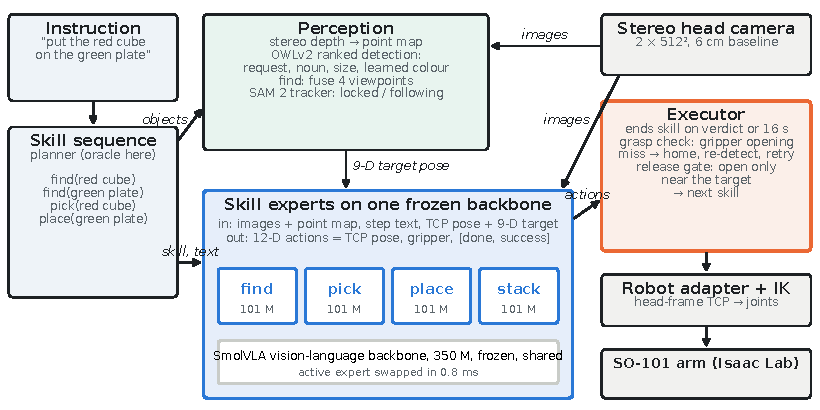
\includegraphics[width=\textwidth]{figures/fig_architecture.pdf}
\caption{System overview. An instruction becomes a sequence of skill calls. Perception turns the stereo images into a
tracked 9-D target pose for the active skill. Each skill is an expert (101\,M trainable parameters) on one frozen,
shared vision-language backbone; only the active expert's weights are swapped. The executor ends skills on the
expert's verdict, checks the grasp from the gripper opening (retrying a missed pick) and gates the release; a
robot adapter and IK map head-frame TCP commands to the arm.}
\label{fig:architecture}
\end{figure*}
\paragraph{Overview.}
Figure~\ref{fig:architecture} shows the system. An instruction (``put the red cube on the green plate'') is mapped to a sequence of skill calls:
\texttt{find(cube)}, \texttt{find(plate)}, \texttt{pick(cube)}, \texttt{place(plate)}. Each skill is executed by a
VLA expert that receives the left and right images of a stereo head camera, a point map from stereo depth, the
step text, and a 19-D state: the tool-centre-point (TCP) pose (position, 6-D rotation, gripper opening) and the
9-D pose of the skill's target object, all in the head frame. It outputs chunks of 12-D actions: TCP pose, gripper
opening, and a verdict $[\textit{done}, \textit{success}]$. A robot-specific adapter and inverse kinematics map the
head-frame TCP command to joint targets, so the experts do not depend on the arm.

\paragraph{Skill experts on a shared backbone.}
All experts share one frozen SmolVLA vision-language backbone (350\,M parameters); each skill has its own
action expert and depth branch (101\,M trainable parameters). Switching skills swaps only these weights
(0.8\,ms). The skills are \texttt{find} (move until the object is clearly visible), \texttt{pick},
\texttt{place} and, added later, \texttt{stack}.

\paragraph{Perception and target poses.}
OWLv2~\cite{minderer2023owlv2} proposes candidate boxes; each candidate is scored by detector confidence for the
request and for the noun, a stereo size likelihood, and a learned colour posterior of the object's own pixels
(one CIELab Gaussian per colour name, fitted on rendered training images; the hand-crafted HSV rules it replaces
scored a rendered brown plate at 0.00). Depth comes from a stereo network~\cite{wen2025foundationstereo}. The
target's yaw is folded by the object's symmetry (90$^\circ$ for cubes): giving the policy the unfolded yaw it was
trained on, but perception cannot measure, dropped pick success from 64\% to 18\%. \texttt{find} fuses detections
from the find view and three preset viewpoints; afterwards a SAM~2~\cite{ravi2024sam2} tracker per object, with a
locked/following state machine on trusted measurements, publishes the target during execution.

\paragraph{Executor.}
A skill ends when the expert reports \textit{done} on two consecutive current-frame readings, or after 16\,s.
After \texttt{pick}, a \emph{grasp check} reads the gripper opening: closed on nothing reads 0.00--0.01, holding a
cube $\approx$0.10. On a miss the executor opens, returns home, re-detects the cube and retries (up to twice).
During \texttt{place}, a \emph{release gate} suppresses any opening command while the TCP is more than 4\,cm
sideways or 6.5\,cm above the perceived target.

%======================================================================
\section{Experimental Setup}\label{sec:setup}
%======================================================================
\begin{figure*}[t]
\centering
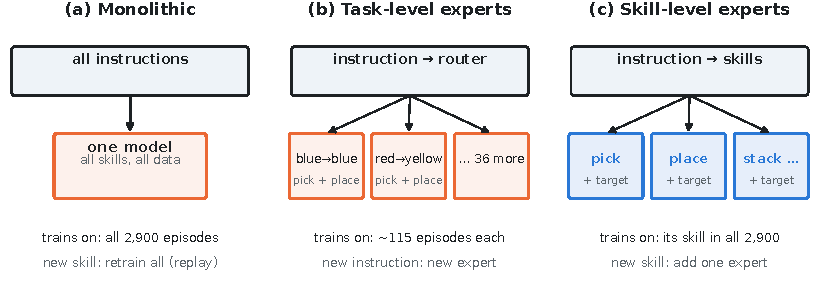
\includegraphics[width=\textwidth]{figures/fig_organisation.pdf}
\caption{Three organisations of the same capacity, data and compute. (a) One model for all instructions and skills.
(b) One expert per instruction, selected by a router, each trained only on its instruction's episodes (CORAL-style
granularity). (c) One expert per skill, composed by a planner and told its target by perception; each expert trains on
that skill's segment of every episode.}
\label{fig:organisation}
\end{figure*}
\paragraph{Environment.}
A simulated SO-101 arm (5-DoF + gripper) in Isaac Lab~\cite{mittal2023orbit} with four 3\,cm cubes and two plates
whose colours are drawn per episode from nine colours (including the cube colours). The stereo head
(2$\times$512$^2$, 6\,cm baseline) is mounted like a human head relative to the arm. Pushes: the target cube is
slid 3--6\,cm during the pick approach.

\paragraph{Data.}
A scripted expert with DART-style noise~\cite{laskey2017dart} generates 1000 static and 1000 moving-target
pick-and-place demonstrations, 500 in which the cube moves during the descent, and 400 failure demonstrations
(grasp miss or slip, off-plate release, drop) whose motion before the failure is masked from the loss so that
only the verdict is learnt there; in total 2{,}900 episodes (563k frames). Recording continues through the release
so that the success label covers frames with the gripper open (\S\ref{sec:reliability}). Training targets imitate
the tracker: detection noise, update rate, dead-band and freezing near the gripper.

\paragraph{Training.}
All models are trained with LeRobot~\cite{cadene2024lerobot} using the same recipe (batch 32, frozen backbone, cosine schedule) from the same base.
Skill experts: 15k steps each for pick and place; find: 15k steps on 1{,}200 find demonstrations.

\paragraph{Protocol.}
Every evaluation uses the same seeded scene sequence, so conditions are paired episode by episode; we report
success rates and two-sided sign tests on the discordant pairs. Even with seeding, about 8\% of individual
outcomes differ between identical runs (GPU non-determinism), so we treat differences of a few episodes as noise.
\emph{Pick} = cube lifted; \emph{full} = cube resting on the target and released.

%======================================================================
\section{Results}
%======================================================================

\subsection{Reliability: where the failures were}\label{sec:reliability}
Before comparing organisations, we brought the system to a reliable baseline by analysing every failure.
Table~\ref{tab:reliability} lists the changes in order. The largest gains came from the executor and the data,
not from the models: an 8\,s skill limit ended episodes whose pick verdict arrived late; demonstrations stopped
when the cube first touched the plate, so the \textit{success} label covered frames with the gripper still closed
and the place expert reported success before releasing; a learned success verdict passed many missed grasps
(68\% accuracy under pushes), whereas the gripper opening separated them almost perfectly; and the place expert
occasionally loosened its grip mid-carry. From the 9-Oct baseline to the final system, full success rose from
45\% to 91\% (71 vs.\ 3 discordant episodes, $p<10^{-17}$) and under pushes from 22\% to 87\%.

\begin{table}[t]
\centering\small
\caption{Reliability changes, cumulative (150 seeded episodes per row; full pick-and-place success).}
\label{tab:reliability}
\resizebox{\columnwidth}{!}{%
\begin{tabular}{lcc}
\toprule
Change & Stationary & Push \\
\midrule
Baseline (fused find, 8\,s skills) & 45\% & 22\% \\
Skill time limit 16\,s & 57\% & -- \\
+ open gripper after place verdict & 64\% & -- \\
+ learned colour posterior (all three) & 72\% & 33\% \\
Retrain: post-release labels, late-push demos & 77\% & 29\% \\
+ grasp check and pick retry & 85\% & 80\% \\
+ release gate (final) & \textbf{91\%} & \textbf{87\%} \\
\bottomrule
\end{tabular}}
\end{table}

\subsection{Experiment 1: one model or one expert per skill?}\label{sec:exp1}
We train a single model on exactly the frames the pick and place experts saw (with the same per-segment
labelling) for 30k steps, matching the 2$\times$15k steps of the two experts. Table~\ref{tab:exp1} shows no
consistent advantage: the monolith is slightly better on stationary scenes and slightly worse under pushes; only
the push pick difference reaches $p<0.05$. \textbf{Splitting by skill does not, by itself, make skills better.}

\begin{table}[t]
\centering\small
\caption{Experiment 1: monolithic vs.\ per-skill experts, same data and compute (150 paired episodes).}
\label{tab:exp1}
\resizebox{\columnwidth}{!}{%
\begin{tabular}{lccc}
\toprule
& Monolithic & Skill experts & sign test \\
\midrule
Stationary pick & 94\% & 91\% & \pv{0.13} \\
Stationary full & 93\% & 91\% & \pv{0.22} \\
Push pick & 81\%$^\dagger$ & 87\% & \pv{0.04} \\
Push full & 81\% & 87\% & \pv{0.12} \\
\bottomrule
\end{tabular}}\\[2pt]
{\footnotesize $^\dagger$2 further picks were confirmed only in the final check (logging fixed later): 82\%.}
\end{table}

\begin{figure*}[t]
\centering
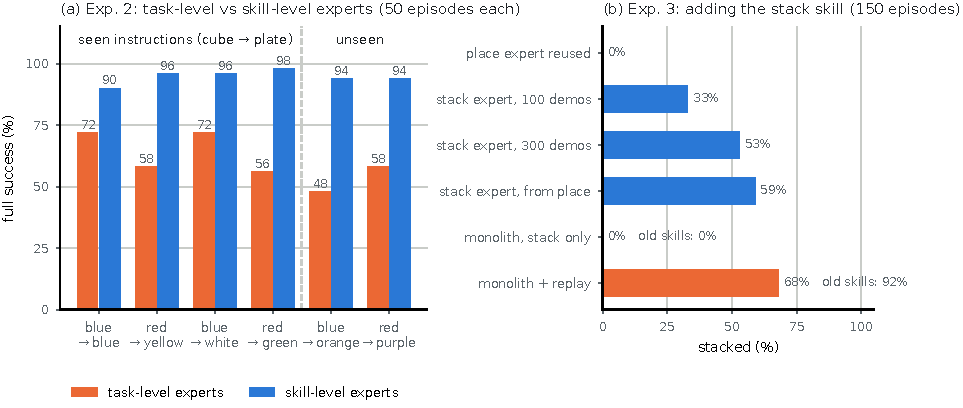
\includegraphics[width=\textwidth]{figures/fig_results.pdf}
\caption{(a) Experiment~4: full success of task-level and skill-level experts on four seen and two unseen
instructions (50 paired episodes each; all differences $p\le0.02$). (b) Experiment~2: stacking success when the
\texttt{stack} skill is added in different ways (150 paired episodes); for the monolith, the success on its original
pick-and-place task afterwards is given.}
\label{fig:results}
\end{figure*}

\subsection{Experiment 4: task-level vs.\ skill-level experts}\label{sec:exp4}
We train four task experts, each a complete pick-and-place model on the 110--121 episodes of one instruction, for
7.5k steps each (30k total, as in Exp.~1), and evaluate each on 50 episodes of its own instruction alongside the
skill experts (same scenes). For two unseen instructions we route to the expert with the same cube colour
(Table~\ref{tab:exp4}, Fig.~\ref{fig:results}a). Skill experts reach 90--98\% on seen and 94\% on unseen instructions; task experts reach
56--72\% even on their own instruction and 48--58\% on unseen ones (all $p\le0.02$). Task experts do not collapse on
unseen instructions, which we attribute to the grounded target pose. \textbf{Organising experts by skill lets each
expert use all the data; organising by task partitions it.}

\begin{table}[t]
\centering\small
\caption{Experiment 4: full success, 50 paired episodes per instruction. Task experts are trained only on their
instruction; for unseen instructions, the expert with the same cube colour is used.}
\label{tab:exp4}
\resizebox{\columnwidth}{!}{%
\begin{tabular}{llccc}
\toprule
& Instruction & Task exp. & Skill exp. & sign test \\
\midrule
\multirow{4}{*}{seen} & blue cube $\to$ blue plate & 72\% & 90\% & \pv{0.02} \\
& red cube $\to$ yellow plate & 58\% & 96\% & \pv{2\cdot10^{-5}} \\
& blue cube $\to$ white plate & 72\% & 96\% & \pv{5\cdot10^{-4}} \\
& red cube $\to$ green plate & 56\% & 98\% & \pv{6\cdot10^{-6}} \\
\midrule
\multirow{2}{*}{unseen} & blue cube $\to$ orange plate & 48\% & 94\% & \pv{2\cdot10^{-6}} \\
& red cube $\to$ purple plate & 58\% & 94\% & \pv{4\cdot10^{-5}} \\
\bottomrule
\end{tabular}}
\end{table}

\subsection{Experiment 2: adding a new skill}\label{sec:exp2}
We add \texttt{stack} (place a cube on another cube), a geometrically different target, from 300 new
demonstrations (Table~\ref{tab:exp2}, Fig.~\ref{fig:results}b). A new stack expert, trained in isolation, stacks 53\% (33\% with 100
demonstrations, $p<10^{-4}$), and 59\% when initialised from the place expert. The existing place expert used
for stacking without training fails entirely: it lowers the cube as onto a plate and knocks it out of the
gripper. Fine-tuning the monolith on the stack data alone erases its previous skills (0\% on stacking and on its
original pick-and-place task); fine-tuning with replay~\cite{rolnick2019replay} of 290 old episodes reaches 68\% stacking and retains
pick-and-place at 92\% (vs.\ 93\%, $p=0.69$). Training compute is identical (5k steps); the difference is
operational. \textbf{The skill expert is added without old data and cannot affect deployed skills; the monolith
transfers more but must be retrained with the old data and re-validated on every change.}

\begin{table}[t]
\centering\small
\caption{Experiment 2: adding \texttt{stack} (150 paired episodes; 5k training steps where trained).}
\label{tab:exp2}
\resizebox{\columnwidth}{!}{%
\begin{tabular}{lcc}
\toprule
Method & Stacked & Old pick+place \\
\midrule
Place expert reused, no training & 0\% & unchanged \\
Stack expert, 100 demos & 33\% & unchanged \\
Stack expert, 300 demos & 53\% & unchanged \\
Stack expert, 300 demos, from place & 59\% & unchanged \\
Monolith, fine-tuned on stack only & 0\% & 0\% \\
Monolith, fine-tuned with replay & \textbf{68\%} & 92\% \\
\bottomrule
\end{tabular}}
\end{table}

\subsection{Experiment 3: composed multi-step tasks}\label{sec:exp3}
We evaluate three compositions that never occur as training episodes, each with 50 seeded episodes and the oracle
skill sequence, so that only execution is compared: \emph{two plates} (two cubes onto the two plates),
\emph{plate-stack} (a cube onto a plate, then a second cube stacked on it) and \emph{tower} (a three-cube tower).
The skill condition uses the pick, place and find experts with the place-initialised stack expert; the monolithic
condition is the monolith fine-tuned with replay, which performs all skills. Success requires every sub-task to be
on target in the final scene.

\begin{figure*}[t]
\centering
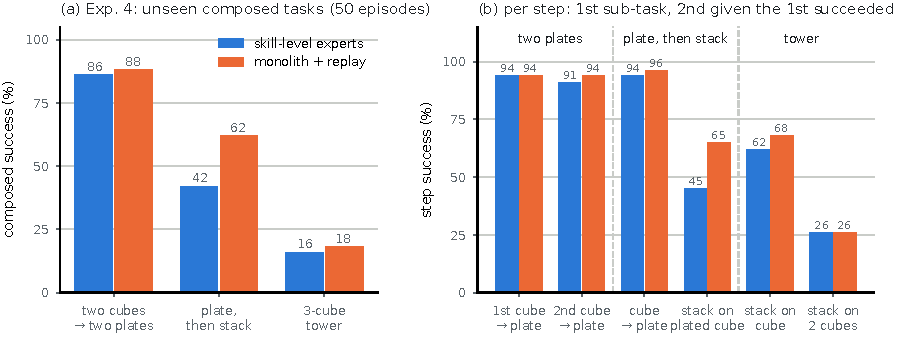
\includegraphics[width=\textwidth]{figures/fig_composed.pdf}
\caption{Experiment~3. (a) Composed success on three unseen multi-step tasks (50 paired episodes each). (b) Success
of each step: the first sub-task, and the second given that the first succeeded. Pick-and-place steps compose
almost independently; stacking onto raised targets (a cube on a plate, a two-cube tower) is the bottleneck.}
\label{fig:composed}
\end{figure*}

\begin{table}[t]
\centering\small
\caption{Experiment 3: composed success (50 paired episodes) and step success (second step given the first).}
\label{tab:exp3}
\resizebox{\columnwidth}{!}{%
\begin{tabular}{lccc}
\toprule
Task & Skill experts & Monolith+replay & sign test \\
\midrule
two plates & 86\% & 88\% & \pv{1.0} \\
plate-stack & 42\% & 62\% & \pv{0.08} \\
tower & 16\% & 18\% & \pv{1.0} \\
\midrule
\multicolumn{4}{l}{\emph{second step given the first}} \\
2nd cube $\to$ plate & 91\% & 94\% & \\
stack on a cube on a plate & 45\% & 65\% & \\
stack on a two-cube tower & 26\% & 26\% & \\
\bottomrule
\end{tabular}}
\end{table}

Table~\ref{tab:exp3} and Fig.~\ref{fig:composed} show three effects. First, pick-and-place steps compose almost
independently: with 94\% on the first step and 91--94\% on the second, both approaches complete 86--88\% of the
two-plate tasks, close to the product of the step rates. In no episode did a later step disturb an earlier
completed one. Second, the composite rate is limited by the weakest skill: on plate-stack the first step succeeds
in 94--96\% of episodes for both, and the gap (42\% vs.\ 62\%, $p=0.08$) comes entirely from the stacking step, in
line with Exp.~2. Third, stacking onto raised targets degrades for both approaches: stacking on a cube that rests
on a plate drops to 45\%/65\%, and stacking on a two-cube tower to 26\% for both, against 59\%/68\% on the table
(Exp.~2). Those target heights never occur in the stacking demonstrations, so neither organisation extrapolates in
height. \textbf{Composition itself works for both organisations; composite success is bounded by the individual
skills, and both fail to extrapolate a skill to target geometry outside its demonstrations.}

%======================================================================
\section{Discussion and Limitations}
%======================================================================
\paragraph{What modularity buys.}
In our setting skill-level experts do not improve the accuracy of individual skills (Exp.~1), but they generalise
across objects and instructions far better than task-level experts at equal compute (Exp.~4), and they allow new
skills to be added safely (Exp.~2). Their cost is reduced transfer between skills: a monolith trained with replay
stacks better than an isolated stack expert, and warm-starting the new expert from a related one recovers part
of the gap. The same difference carries over to composed tasks (Exp.~3), where composite success follows the weakest
skill.

\paragraph{The role of grounding.}
The target pose is what makes a single pick expert serve every object, and it also keeps task experts from failing
completely on unseen instructions. It does not transfer across target \emph{geometry}: a place expert cannot stack.

\paragraph{Reliability.}
The largest end-to-end gains came from executor mechanisms and labelling, and several apparent model failures
were evaluation or labelling artefacts (a simulator time-out that silently reset long episodes; a success label
placed before the release). We encourage reporting per-cause failure accounting alongside success rates.

\paragraph{Limitations.}
All results are in simulation, with one arm and one family of objects (cubes and plates). Our task-level condition
re-implements the granularity of CORAL~\cite{luo2026coral} rather than the method itself. The planner is an oracle
in the experiments. We have not yet evaluated on a standard benchmark such as LIBERO~\cite{liu2023libero} or on
real hardware; both are the next steps.

%======================================================================
\section{Conclusion}
%======================================================================
We studied at which granularity to define experts on a shared VLA backbone. Defining them per skill and grounding
each skill in a tracked target pose gave much better generalisation than per-task experts, no loss against a
monolithic model, and safe extension with new skills; executor-level mechanisms were as important as the models
for end-to-end reliability. Composed tasks succeed when their skills do: composition itself added no failures,
which makes the remaining gap a matter of individual skills and their training distribution.

\bibliographystyle{IEEEtran}
\bibliography{references}

\end{document}
